\chapter{Mathematical introduction}
The modern approach to the closed system dynamics is using differential geometry formalism. Before we get to the quantum mechanics itself, lets define the formalism and recapitulate some definitions of this branch of mathematics. More detailed notes can be found for example in \citep{fecko}.

Let's have a manifold $\M$ and curves 
$$\gamma:\R \overset{open}{\supset} I \rightarrow \M \qquad \xi\mapsto \gamma(\xi).$$ 
The space of functions is $\F(\M)\equiv\{f:\M\rightarrow \R\}$, where 
$$f:\M\rightarrow U\overset{open}{\subset} \R \qquad x\mapsto f(x).$$
To define \emph{vectors} on $\M$, we need to make sense of the \emph{direction}. It is defined using curves satisfying 
$$\gamma_1(0)=\gamma_2(0)\equiv P$$
$$\der{}{t}x^i(\gamma_1(t))\big|_{t=0}=\der{}{t}x^i(\gamma_2(t))\big|_{t=0}.$$
Taking the equivalence class created by those two rules, sometimes noted as $[\gamma]=v$, we have element of the tangent space to $\M$. We will use standard notation for the tangent space to $\M$ in some point $xP$ as $\T_P\M$ and contangent space as $\T^*_P\M$. Unifying all those spaces over all $x$ we get tangent and cotangent bundle, $\TT\M$ and $\TT^*\M$ respective. To generalize this notation to higher tensors, we denote $\T_P\M\in \TT^1\M$, $\T^*_P\M\in \TT_1\M$, thus the space of $p-$times contravariant and $q-$times covariant tensors is denoted $\TT^p_q\M$.

Using the congruence of the curves on $\M$, the expression 
\begin{equation}
    \der{}{\xi}f\circ \gamma(\xi)\Big|_{\xi=0}
\end{equation}
has a good meaning and we can define the \emph{derivative} in some $P\in\M$ as
\begin{equation}
    \bm v: \F(\M)\rightarrow \R \qquad f\mapsto \bm v[f]\equiv \frac{\d f(\gamma(\xi))}{\d \xi}\Big|_P \equiv \partial_\xi\Big|_P f .
\end{equation}
It holds, that $\bm v\in \T_P\M$ and can be expressed as the \emph{derivative in direction},\footnote{
        The direction itself is usually denoted as
        \begin{equation}
            \frac{\D}{\d\bm\alpha}\gamma(\xi),
        \end{equation}
        where the big D notation is used to point out that it's not a classical derivative, but it maps curves to some entirely new space of directions.
    } 
which can be understood in coordinates as
\begin{equation}
    \bm v[f] = \der{}{\bm v} f\circ \gamma(\xi)\Big|_{\xi=0}=v^\mu\der{}{x^\mu} f(\bm x)\Big|_{P}.
\end{equation}
The directionnal derivative will be denoted 
$$\nabla_v$$
and in basis $\bm e_i \equiv \partial/\partial x^i$ we will denote 
$$\nabla=(\bm e_x, \bm e_y,\bm e_z).$$



To get some physical application, we need to define one strong structure on manifolds -- differentiable metric tensor $g_{\mu\nu}\in\TT^0_2\M$ -- so the covariant derivatives and parallel transport are well-defined everywhere. 


\section{Fiber bundle}
\label{sec:bundleDef}
We already know tangent and cotangent spaces. Thinking of manifold $\M$ as a fiber, for which at any point $x$ we create new manifold $\T_x\M$, we and unifying all those tangent spaces, we get so-called \emph{vector bundle}. 
\begin{definition}
    Structure $(\mathcal{E},\mathcal{B},\pi,\mathcal{F})$, for topological spaces $\mathcal{E}$ (\emph{total space}), $\mathcal{B}$ (\emph{base space}), $\emph{F}$ (\emph{fibre}) and a continuous surjection $\pi: \mathcal{E}\rightarrow \mathcal{B}$ satisfying a local triviality\footnote{local triviality} is called a \emph{Fiber bundle} (\emph{projection map}). In addition, the $\mathcal{B}$ is assumed to be connected\footnote{can't be represented as a union of two disjoint sets} and for every $x\in \mathcal{B}$, there is an open neighborhood $\mathcal{U}\subset \mathcal{B}$ (\emph{trivializing neighborhood}) such that there exists a homeomorphism from $\mathcal{U}$ to so-called \emph{product space}
    $$\phi: \pi^{-1}(\mathcal{U})\rightarrow \mathcal{U}\times \mathcal{F},$$
    such that $\pi^{-1}\pi(\mathcal{U})=\mathcal{U}$.
\end{definition}

The above mappings can be more clear from figure \ref{fig:bundle}. Because projections of products are open maps, $\pi: \mathcal{E}\rightarrow \mathcal{B}$ must be open map.
\begin{figure}[h]
    \centering
    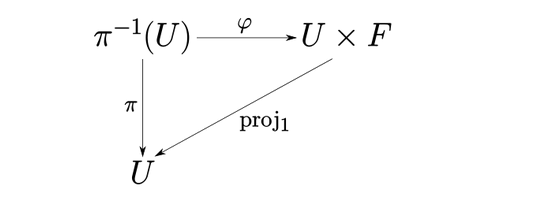
\includegraphics[width=0.5\textwidth]{../img/bundle.png}
    \caption{Mappings needed for the bundle definition.}
    \label{fig:bundle}    
\end{figure}
The meaning of definition is, that manifolds at every point $x\in \mathcal{F}$ are all locally diffeomorphic to each other.
\section{Vector Bundle}
\textcolor{red}{Conversely, given a fiber bundle (E, X, $\pi$, Rk) with a GL(k) cocycle acting in the standard way on the fiber Rk, there is associated a vector bundle. This is sometimes taken as the definition of a vector bundle}


\subsection{Connection on vector bundles}
\citep{lu}[chap. 10.1]
Connection maps vector from tangent space to base manifold $\mathcal{X}$ with some element from total space $\mathcal{E}$ to total space
$$\Gamma: \mathcal{X}\times \mathcal{E}\rightarrow \mathcal{E}$$
such, that
\begin{itemize}
    \item $\Gamma_X s$ is $\mathcal{F}-$linear in $X$ and $\R-$linear in $s$
    \item Leibniz rule for $f\in \mathcal{C}^\infty$ is satisfied: $\Gamma_X(f s) = (X f)s+f\Gamma_X s$
\end{itemize}


\subsection{Metric on vector bundles}
Map
$$g_{\mu\nu}: \mathcal{B}\times \mathcal{B} \rightarrow \R$$

\section{Section}
\label{sec:section}
\emph{Section} is a function
$$f:\mathcal{B}\rightarrow \mathcal{F},$$
such that $\pi(f(x))=x$ for $\forall x\in \mathcal{B}$. This defines new manifold cutting throw $\mathcal{E}$.

\textcolor{red}{Sectioning of fiber bundles creates vector spaces}


\section{Pull-back and push forward}
Push-forward and pull-back are used to transport vectors and covectors between manifolds. Let's have two manifolds $\M$, $\mathcal{N}$, a smooth mapping $\phi$ and functions $f,\tilde f$ such that
\begin{align*}
    \phi&:\M\rightarrow \mathcal{N}\qquad x\mapsto \phi x\\
    \tilde f&:\mathcal{N}\rightarrow \R 
\end{align*}
\emph{Pull-back of the function} then defines a new function $
f:\M\rightarrow \R $ as
$$\phi^*:\F \mathcal{N}\rightarrow \F\M \qquad  \tilde f\mapsto f=(\phi^*\tilde f)(x)\equiv \phi^*\tilde f(x) =\tilde f(\phi x).$$
\emph{Push-forward of a vector} is defined as
$$\phi_*: \T_x\M \rightarrow \T_{\phi x}\mathcal N\qquad \phi_* 
\Der{\gamma(\xi)}{\xi}\Big|_x=\Der{\phi \gamma(\xi)}{\xi}\Big|_x$$
and \emph{pull-back of a covector} $\bm\tilde\alpha\in \T_{\phi x}\mathcal N$ is
$$\phi^*: \T_{\phi x}\mathcal N\rightarrow \T_x\M  \qquad (\phi^*\bm \tilde\alpha)_\mu v^\mu\big|_x= \tilde\alpha_\mu (\phi_* \bm v)^\mu\big|_{\phi x}.$$
If $\phi$ has a smooth inversion, i.e. it is a dippheomorphism, we can define pull-back of vectors as
\begin{equation}
    \phi^*=\phi_*^{-1}
\end{equation}
and push-forward of covectors
\begin{equation}
    \phi_*=(\phi^{-1})^*
\end{equation}

\section{Flow}
% Flow is
% \begin{equation}
%     \phi_*\in \textrm{Diff}\M
% \end{equation}
\section{Covariant derivative and parallel transport}
\textcolor{blue}{this section is probably not needed}


Covariant derivative is generally\dots
Metric covariant derivative is\dots

Parallel transport of vector $\bm v\in \T_p \M$ will be denoted $\Par_\gamma \bm v\in \T_{}$

Affine connection can be expressed as
\begin{equation}
    \Gamma^{\alpha}_{\mu\nu} = \frac{1}{2}g^{\alpha \beta}\left(g_{\beta\mu,\nu}+g_{\nu\beta,\mu}-g_{\mu\nu,\beta}\right),
\end{equation}
where we used comma notation for the coordinate derivative.
The covariant derivative of $\bm a\in \T_P\M$ is then defined
\begin{equation}
    \Der{a^\mu}{x^\nu}=a_{\;,\nu}^\mu-\Gamma^\mu_{\alpha\beta} x^\alpha a^\beta 
\end{equation}
and for $\bm\alpha\in \T_P^*\M$ it is
\begin{equation}
    \Der{\alpha_\mu}{x^\nu}=\alpha_{\mu,\nu}-\Gamma^\alpha_{\mu\beta}x^\beta \alpha_\alpha 
\end{equation}

The vector $v\in \T_P\M$ is said to be parallel transported along curve $\gamma(\lambda)$, if it's covariant derivative
\begin{equation}
    \Der{v^\mu}{\xi}=0
\end{equation}
vanishes along $\gamma$.

\section{Parallel transport on vector bundles}
\textcolor{blue}{this is what we need}
Parallel transport of vector $V$ along curve $\gamma$ will be denoted
$$\Par_\gamma V.$$
It is 


\section{Antisymmetric tensors and wedge product}
p-form $A\in \TT_p \M$ is called \emph{antisymmetric}, if changing the order of the indices has impact only on the sign, symbolically
$$A_{i_1\dots i_p} = \sign(\sigma)A_{i_{\sigma_1}\dots i_{\sigma_p}},$$
where $\sigma$ is some permutation.\emph{Antisymmetrisation} is defined as a normalized sum over all permutation
\begin{equation}
    A^{[i_1\dots i_p]}\equiv \frac{1}{p!}\sum_\sigma A^{[i_{\sigma_1}\dots i_{\sigma_p}]}. 
\end{equation}

The \emph{wedge product} of $A\in \TT_p \M$ and $B\in \TT_q \M$ is antisymmetrisation of the tensor product in the sense
\begin{equation}
    A\wedge B\equiv \frac{(p+q)!}{p!q!} A^{[i_1\dots i_p}\otimes B^{i_1\dots i_q]}
\end{equation}
